\section{Fundamentals of Particle Image Velocimetry}

Particle Image Velocimetry, or PIV, is a class of methods employed by 
experimental fluid mechanics to measure instantaneous vector velocity fields by 
measuring the displacements of small visible particles which follow the motion 
of the fluid \cite{adrian2011}. Figure \ref{fig:quiver_example} shows a typical 
resulting vector field from measurements of a vortical flow. Each of these 
two-dimensional vectors was measured simultaneously in a thin sheet of fluid. 
The velocity of the fluid is sensed by acquiring images of well entrained 
particles at precise times and measuring the displacement of those particles. 
This is accomplished with the use of cameras for acquiring images and an 
intense laser to illuminate particles within the desired plane. 
This technique can be used to study flows in gases and liquids, and is derived 
from techniques originally developed to measure deformations on the surface of 
solid material.

\begin{figure}[H]
	\centering
	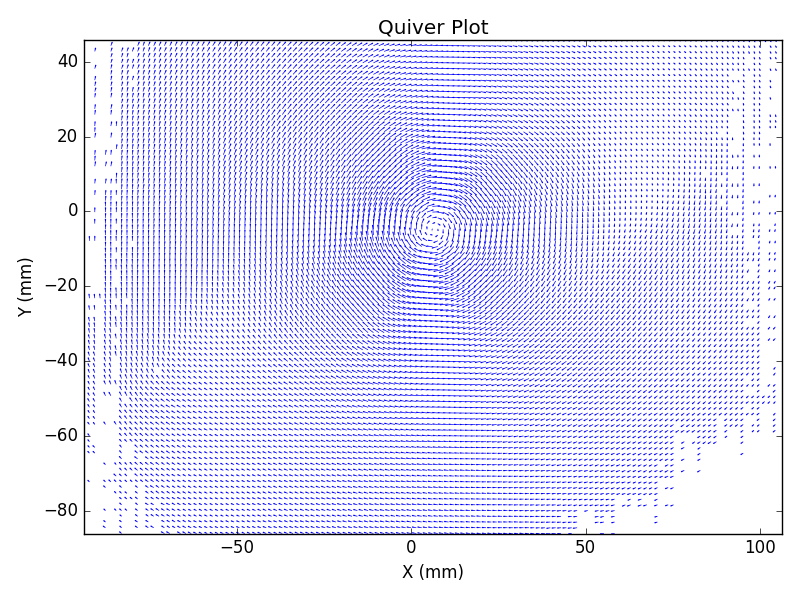
\includegraphics[width=5in]{figs/example_vortex_figs/example_quiver}
	\caption{Velocity vector field of a vortical flow structure as produced by 
	PIV.}
	\label{fig:quiver_example}
\end{figure}

 
\subsection{The Case for PIV}

Unlike other flow measurement techniques, PIV is a non-invasive method to 
directly measure time and displacement, and thus velocity. PIV is also capable 
of resolving vector measurements at many positions within a two dimensional 
slice of the flow field simultaneously, while other measurement techniques 
require taking data at many locations sequentially over a much greater period 
of time. Single camera PIV can measure two components of the velocity vectors 
aligned with the image plane, but the PIV method is capable of resolving many 
dimensions of fluid flow with incremental increases in system complexity. The 
addition of another camera allows the full three dimensional velocity vector to 
be measured, and a sweeping beam laser allows the interrogation of an entire 
volume of flow field instead of a slice.

Stereo PIV is used widely because it provides a full velocity vector, and 
requires only an additional camera, slightly more complex calibration and 
software to process the imagery.  A stereo PIV system with a 
stationary sheet laser can resolve three dimensional velocity vectors and their 
fluctuations within a two dimensional slice of fluid flow. A two point 
correlation tensor containing important information about the turbulent 
structure of a flow can be obtained readily with PIV. The non-invasive nature 
of PIV, combined with the  ability to interrogate a flow volume very quickly 
for information with high dimensionality makes it exceptionally useful in fluid 
mechanics. \cite{adrian1991}

\subsection{Principles of Planar PIV}

A simple planar PIV system consists of a double pulsed laser, light sheet 
forming optics, particle seed, a single lens camera, image digitization 
hardware, and a computer system for data storage and subsequent analysis. The 
underlying concept behind all PIV is that light scattered from the particles as 
they move through the flow field allows a pair of images to capture information 
about the motion of that particle. Double pulsed illumination is commonly used 
in PIV systems due to its relatively low cost and complexity compared with 
multiple laser source systems. The energy required to adequately illuminate an 
area of interest depends upon the size of that area, and the scattering 
properties of the particle seed. Solid state Nd:YAG lasers are typically used 
for this purpose \cite{adrian2011}. An $(X, Y, Z)$ coordinate system 
is defined 
within the light sheet that exists in $(X, Y)$ space, and relates linearly to a 
coordinate system in the image plane of the camera in $(X_p, Y_p)$ pixel space. 
At a time $t$, a laser light sheet is produced for a short pulse and the camera 
captures an image of the light scattering from particles within the flow. At 
some short time later, $t + dt$, a second pulse occurs and a second image is 
taken. By measuring the pixel displacements $(\Delta X_p, \Delta Y_p)$ for a 
particle in the image plane, and transforming the coordinates into the plane of 
the laser one obtains $(\Delta X, \Delta Y, \Delta Z)$. This coordinate 
transform can be obtained from precise information about the optical geometry 
of the system, or by direct measurement of calibration data \cite{fouras2007}.
The method of direct measurement of a calibration target was used in this 
research. 

The detection rate, accuracy, and reliability of PIV depends upon careful 
selection of experimental parameters. Kean and Adrian suggest a set of six 
important dimensionless quantities and ideal operating ranges that improve the 
chances of high quality PIV results . The parameters 
are data validation criterion, particle image density, relative in-plane image 
displacement, relative out-of-plane displacement, velocity gradient, and the 
ratio of the mean image diameter to the interrogation spot diameter 
\cite{kean1990,kean1991}. Steep velocity gradients create random errors as the 
individual particle displacements cover a discreet range within an 
interrogation spot. Particle displacements should be restricted to 25\% of the 
interrogation spot diameter for in-plane velocities, and to 25\% of the light 
sheet thickness in out-of-plane velocities. One way to mitigate both of these 
effects is to use as high resolution PIV as possible, or by scaling the 
interrogation area down by altering the zoom of the cameras. Since the velocity 
profile of an axial vortex can contain high velocity gradients in the vicinity 
of the core, and both in-plane and out-of-plane velocities are expected to be 
high, the present experiments used 50mm lenses to zoom each camera to 
focus on a small an interrogation plane as possible.

\subsection{Principles of Stereo PIV}

Classical single camera PIV is only capable of capturing the projection of the 
velocity vector on the image plane. The out-of-plane component is lost 
completely, and the in-plane components are affected by unrecoverable error. In 
Stereo PIV, a pair of cameras may obliquely view the same plane and the entire 
3d velocity vector may be inferred using the camera geometry. This technique 
includes tilting the backplanes of the cameras to satisfy the Scheimpflug image 
criteria and a dewarping function based on camera geometry to account for 
projective distortion \cite{willert1997}. An example of the geometric set up 
used by Willert to study the movement of a ring vortex through the 
interrogation plane is shown in Figure \ref{fig:stereo_piv}. Uncertainties 
associated with high out-of-plane motion in planar PIV are greatly reduced in 
stereo PIV.

\begin{figure}[H]
	\centering
	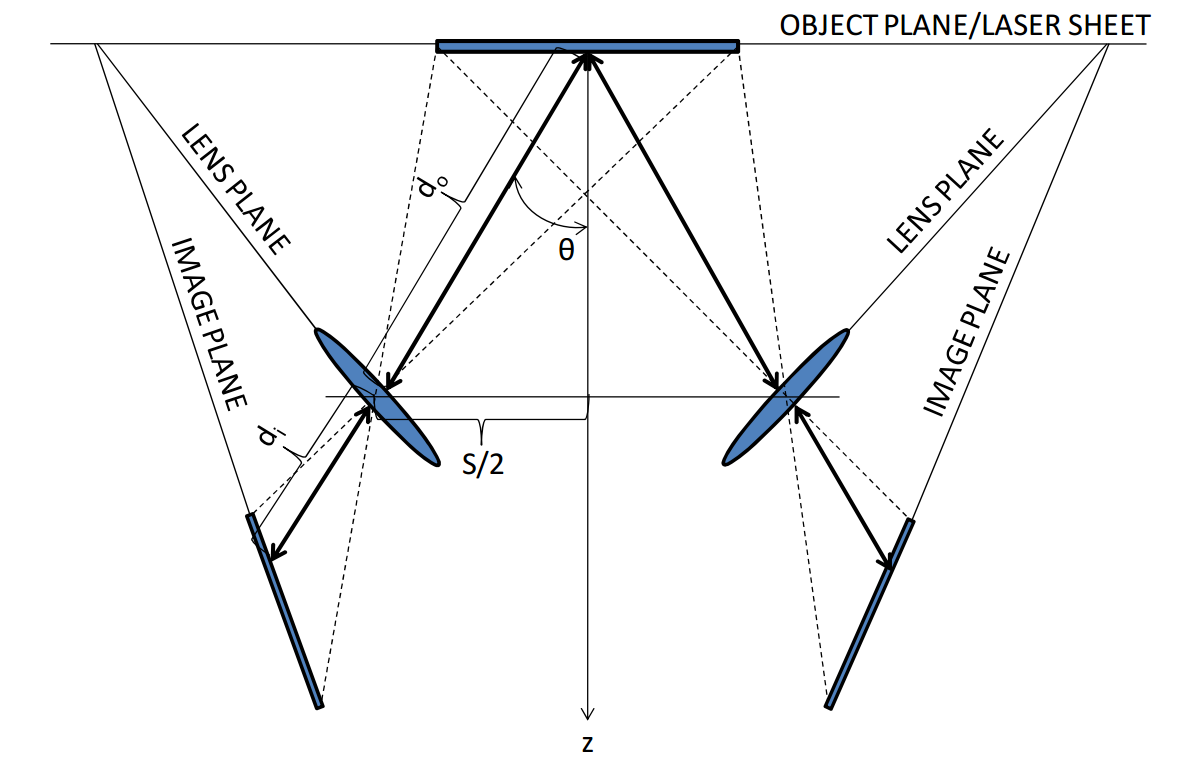
\includegraphics[width=5in]{figs/piv_method/stereo_piv_optics}
	\caption{Stereo camera PIV system for mapping three dimensional velocity 
		vectors}
	\label{fig:stereo_piv}
\end{figure}  

\subsection{Particles}

\subsubsection{Particle Dynamics} 

\subsubsection{Error Due to Slip}

\subsubsection{Seeding Particles for PIV}

\subsection{Image processing}

\cite{soloff1997, willert1997}.

\subsection{Interrogation}

\subsection{Measurement of Fluid Flow}

\subsection{PIV in Three Dimensions}

\subsection{Practical PIV Systems}


